\documentclass{article}
\usepackage[utf8]{inputenc}
\usepackage{hyperref}
\usepackage{tikz}
\usetikzlibrary{automata,positioning}
\usepackage{amsmath}
\usepackage{amssymb}
\usepackage{mathtools}
\usepackage{pgfplots}
\usepackage{float}
\usepackage{multirow}
\usepackage{algorithm2e}
\restylefloat{table}
\usepackage{algpseudocode,algorithm,algorithmicx}
\newcommand*\Let[2]{\State #1 $\gets$ #2}
\algrenewcommand\algorithmicrequire{\textbf{Precondition:}}
\algrenewcommand\algorithmicensure{\textbf{Postcondition:}}
\usepackage{titlesec}
\titleclass{\subsubsubsection}{straight}[\subsection]

\newcounter{subsubsubsection}[subsubsection]
\renewcommand\thesubsubsubsection{\thesubsubsection.\arabic{subsubsubsection}}
\renewcommand\theparagraph{\thesubsubsubsection.\arabic{paragraph}} % optional; useful if paragraphs are to be numbered

\titleformat{\subsubsubsection}
  {\normalfont\normalsize\bfseries}{\thesubsubsubsection}{1em}{}
\titlespacing*{\subsubsubsection}
{0pt}{3.25ex plus 1ex minus .2ex}{1.5ex plus .2ex}
\makeatletter
\renewcommand\paragraph{\@startsection{paragraph}{5}{\z@}%
  {3.25ex \@plus1ex \@minus.2ex}%
  {-1em}%
  {\normalfont\normalsize\bfseries}}
\renewcommand\subparagraph{\@startsection{subparagraph}{6}{\parindent}%
  {3.25ex \@plus1ex \@minus .2ex}%
  {-1em}%
  {\normalfont\normalsize\bfseries}}
\def\toclevel@subsubsubsection{4}
\def\toclevel@paragraph{5}
\def\toclevel@paragraph{6}
\def\l@subsubsubsection{\@dottedtocline{4}{7em}{4em}}
\def\l@paragraph{\@dottedtocline{5}{10em}{5em}}
\def\l@subparagraph{\@dottedtocline{6}{14em}{6em}}
\makeatother

\setcounter{secnumdepth}{4}
\setcounter{tocdepth}{4}
\title{AINT252}
\author{Gabryel Mason-Williams }
\date{February 2019}

\begin{document}
\def\layersep{2.5cm}
\maketitle
\begin{abstract}
    This document contains my lectures notes based on the series of lectures in the AINT252 module given by lectures at The University of Plymouth 
\end{abstract}
\newpage
\tableofcontents
\newpage
%\section{Introduction Lecture}
This lecture covered a quick introduction to the module about AI ending with a formal definition of a simple neural network and types of learning. This lecture was presented by Prof Roman Borisyuk and some of the information is directly copied from the lecture slides.
\subsection{Introduction to AI}
These days, AI is becoming a more and more popular approach for solving many different real-life problems. Since the time of the first computers (1950$^{th}$), AI has been an active scientific discipline.
\\\\
The field of AI draws upon many different interdisciplinary fields such as; computer science, mathematics, information theory, engineering, psychology, cognitive science and many more.
\\\\
AI is a challenging goal in which we want computer code (an agent) to mimic/ have natural intelligence, i.e. a human brain. Alan Turing in his paper "Computing Machinery and Intelligence. Mind 49:433-460 (1050) formulated a question: Can a machine think?. Turing suggested a way to test this would be to use the "imitation game."
\footnote{If you do not want to read the whole paper this overview is very detailed and give the gist of the paper (\href{https://blog.acolyer.org/2017/10/20/computing-machinery-and-intelligence/}{link})}
\subsection{Natural AI}
A simple but attractive idea for designing AI is to look at the human brain as this is the most complex and only thing we know of as General Intelligence which is ultimately our goal with AI, because of this a lot of our models are based on our understanding of how the brain works, i.e. the Biological Neuron.
\subsubsection{Biological Neuron}
A neuron consists of the cell body (soma), input (dendrite) and an output (axon). To communicate between neurons is via the synapse, and the synaptic weight defines the efficacy of this transmission \footnote{This is also known as the connection strength and is adjustable}. A neuronal network is a set of interconnected neurons, and a neuron integrates all the inputs signals and compares the inputs with the threshold: if it exceeds the threshold, then the neuron generates an action potential.
\\\\
We try and mimic this structure in neural networks as you will see in the next section.
\newpage
\subsection{Formal Neural Network}
A basic Neural Network can be written like so, and an example of what this network would look like is shown in figure \ref{fig:NeuralNetwork:4-5-2} \footnote{There is a series of lectures on youtube from 3Blue1Brown covering this topic in great detail (\href{https://www.youtube.com/watch?v=aircAruvnKk&list=PLZHQObOWTQDNU6R1_67000Dx_ZCJB-3pi}{link})}
\begin{itemize}
    \item Inputs: $x_1, x_2,..,x_n$; binary (0/1)
    \item Connection Strengths: $w_1,w_2,...,w_n$ 
    \item Summation $ h = \sum_{i=1}^{n} w_i x_i$
    \item Output $y = f(h)$; binary: if $h > T$ then $y = 0$ else $y =1$
\end{itemize}
Where $f(h)$ is the activation function with a threshold of $T$
\begin{figure}[H]
    \centering
  \begin{tikzpicture}[shorten >=1pt,->,draw=black!50, node distance=\layersep]
    \tikzstyle{every pin edge}=[<-,shorten <=1pt]
    \tikzstyle{neuron}=[circle,fill=black!25,minimum size=17pt,inner sep=0pt]
    \tikzstyle{input neuron}=[neuron, fill=green!50];
    \tikzstyle{output neuron}=[neuron, fill=red!50];
    \tikzstyle{hidden neuron}=[neuron, fill=blue!50];
    \tikzstyle{annot} = [text width=4em, text centered]

    % Draw the input layer nodes
    \foreach \name / \y in {1,...,4}
    % This is the same as writing \foreach \name / \y in {1/1,2/2,3/3,4/4}
        \node[input neuron, pin=left:Input \#\y] (I-\name) at (0,-\y) {};

    % Draw the hidden layer nodes
    \foreach \name / \y in {1,...,5}
        \path[yshift=0.5cm]
            node[hidden neuron] (H-\name) at (\layersep,-\y cm) {};

    % Draw the output layer node
    \node[output neuron,pin={[pin edge={->}]right:Output}, right of=H-2] (O) {};
    \node[output neuron,pin={[pin edge={->}]right:Output}, right of=H-4] (A) {};
    % Connect every node in the input layer with every node in the
    % hidden layer.
    \foreach \source in {1,...,4}
        \foreach \dest in {1,...,5}
            \path (I-\source) edge (H-\dest);

    % Connect every node in the hidden layer with the output layer
    \foreach \source in {1,...,5}
        \path (H-\source) edge (O);
    \foreach \source in {1,...,5}
        \path (H-\source) edge (A);

    % Annotate the layers
    \node[annot,above of=H-1, node distance=1cm] (hl) {Hidden layer};
    \node[annot,left of=hl] {Input layer};
    \node[annot,right of=hl] {Output layer};
\end{tikzpicture}  

    \caption{Neural network:4-5-2}
    \label{fig:NeuralNetwork:4-5-2}
\end{figure}
Neural Network is a set of coupled neurons Similar to real neurons; formal neurons are interconnected: the output of one neuron is an input to another neuron. The figure above demonstrates this.
\subsection{Learning}
Similar to a real neural network, the Artificial Neural Network (ANN) can learn by adjusting the connection strength. The current most popular types of learning in AI: supervised, unsupervised and reinforcement learning 
\\\\
For example, Deep Learning (Deep Neural Network) is a method to learn from the data; Deep Learning can use supervised learning: for a particular input vector, a "teacher" defines a desirable output. Thus, the deep neural network can be trained to find a correspondence between inputs and desirable outputs. 
 


\newpage
%\section{Theoretical basis of AI}
\subsection{AI algorithms for classification}
From a theoretical point of view many AI algorithms are formulated in terms of classification, i.e. a pattern recognition problem can be formulated as a classification problem. 
\\\\
A data set consists from cases (objects) and each case is characterised by some features, each case can be represented by a vector of features such that $\overrightarrow{x} = (x_1,x_2,...,x_p)$  each vector can be considered as a dot in p-dimensional space and all cases together form a cloud. If we Assume that each vector belongs to some class, the number of classes is M. The goal is to find a classifier that assigns to each case a label of some class.
\subsubsection{What a computer can see}
An image classifier takes a single image and assigns probabilities to labels. For an image of size $248\times400$ pixels and three colour channels, the image will consist of 297,600 numbers where each number is an an integer in a range from 0 to 255, our task if turn these numbers into a label.
\subsection{Data pre-processing}
There are four common forms of data pre-processing: centering, normalisation, dimensionality reduction, noise cancelling. To understand these procedure we assume that our data has a random nature and we use probability theory and statistics to deal with random variable and data analysis. 
\\\\
A Data matrix $X$, where we will assume that $X$ is of size $[n,p]$ (where $n$ is the number of data ( cases), $p$ is the dimensionality of the feature vector).

\subsection{Normal distribution}
A continuous random variable $X$ which is bell-shaped and has mean (expectation) $\mu$ and standard deviation $\sigma$ is said to follow a Normal Distribution with
parameters $\mu$ and $\sigma$.
\\\\
In shorthand, $X \sim \mathcal{N}(\mu,\,\sigma^{2})\,.$
This may be given in \emph{standardised} form by using the transformation
\begin{equation}
    z = \frac{z - \mu}{\sigma} \rightarrow x = \sigma z+ \mu \text{, where } Z \sim \mathcal{N}(0,\,1)\,.
\end{equation}
The normal distribution is important because of the Central Limit Theorem which states that a sum of arbitrary random variables will have a distribution that is approximately normal. 
\subsection{Bivariate normal distribution }
The multivariate normal distribution is a generalisation of the univariate normal to two or more variables, Each element of a normally distributed random vector has a univariate normal distribution. In the simplest case there is no correlation among variables, and elements of the vectors are independent univariate normal random variables. 

\begin{figure}[htbp]
    \def\centerx{2}
    \def\centery{-1}
    
    \centering
    \begin{tikzpicture}
        \begin{axis}
        \addplot3[surf,domain=-2:6,domain y=-5:3] 
            {exp(-( (x-\centerx)^2 + (y-\centery)^2)/3 )};
        \node[circle,inner sep=1pt,fill=blue,pin=90:$\mu$] 
            at (axis cs:\centerx,\centery,1) {};
        \end{axis}
    \end{tikzpicture}
    \caption{Bivariate normal distribution 3D perceptive}
    \label{fig:my_label}
\end{figure}
\begin{figure}[htbp]
    \def\centerx{2}
    \def\centery{-1}
    \centering
    \begin{tikzpicture}
        \begin{axis}[view={0}{90},axis equal]
        \addplot3[contour gnuplot,domain=-2:6,domain y=-5:3] 
            {exp(-( (x-\centerx)^2 + (y-\centery)^2)/3 )};
        \node[circle,inner sep=1pt,fill=blue,pin=90:$\mu$] 
            at (axis cs:\centerx,\centery,1) {};
        \end{axis}
    \end{tikzpicture}
    \caption{Bivariate normal distribution 2D perceptive}
    \label{fig:my_label}
\end{figure}
$p$ is the correlation $-1 \leq p \leq 1$ 
\begin{itemize}
    \item $p = 0$ means that the varables are independent
    \item $p = +1$ means that the variables are linearly dependent
    \item $p = -1$ means also the linear dependence but the increase of one variable is associated with the decrease of an other.
\end{itemize}
\subsection{Statistics: Random sample}
Statistics is an interface between the probability theory and data, it provides multiple procedures for data analysis. In statistics the data set is a sample, this sample should be chosen in a proper way and correctly represent a random variable which we would like to estimate.
\subsection{Parameter estimators}
Data analysis is based of statistical estimator of the random variable $X$, i.e. for sample $X = (x_1,x_2,...,x_n)$, 
\\\\
The estimator of the mean is
\begin{equation}
  \Bar{X} = \frac{1}{n}\sum_{i=1}^{n} x_i.
\end{equation}
The estimator of the variance is 
\begin{equation}
  S_x^2 = \frac{1}{n} {\sum_{i=1}^{n} (x_i - \Bar{X})^2}.
\end{equation}
The estimator of the standard deviation is 
\begin{equation}
    S_x = \sqrt{\frac{1}{n} {\sum_{i=1}^{n} (x_i - \Bar{X})^2}}
\end{equation}
Now consider the bivariate random variable $(X,Y) = \{(x_i,y_i)\},i = 1,2,...,n$
\\\\
The estimator of the covariance is 
\begin{equation}
    cov(X,Y) = \frac{1}{n-1} {\sum_{i=1}^{n} (x_i - \Bar{X})}(y_i - \Bar{Y})}
\end{equation}
The estimator of the correlation is 
\begin{equation}
    p = \frac{cov(X,Y)}{S_x S_y}
\end{equation}
\subsection{Data Centering}
Mean subtraction is the most common form of pre-processing, it involves subtracting $\mu$ across every individual feature in the data and has the geometric interpretation of centering the cloud of data around the origin along every dimension. 
\subsection{Data normalisation}
Normalisation referees to normalising the data dimensions so that they are approximately the same scale. There are two common ways of achieving this normalisation
\begin{enumerate}
    \item To divide each dimension by its standard deviation, once it has been zero centered
    \item normalised each dimension so that the min and max along the dimension is -1 and 1 respectively
\end{enumerate}
It only makes sense to apply this pre-processing if you have a reason to believe that different input features have different scales, but thy should be approximately equal importance to the learning algorithm. In the cases of images the relative scales of pixels are already approximately equal, so it is not strictly necessary to perform this addition pre-processing step.
\subsection{Dimensionality reduction: Principal Component Analysis (PCA)} 
Principal components analysis is a quantitatively rigorous method for achieving data simplification and dimensionality reduction. The method generates a new set of variables, called principal components.  Each principal component is a linear combination of the original variables. All the principal components are orthogonal to each other, so there is no redundant information. The principal components as a whole form an orthogonal basis for the space of the data.
\begin{enumerate}
    \item The first principal component is a single axis in space. When you project each observation on that axis, the resulting values form a new variable. The variance of this variable is the maximum among all possible choices of the first axis. 
    \item The second principal component is another axis in space, perpendicular to the first. Projecting the observations on this axis generates another new variable. The variance of this variable is the maximum among all possible choices of this second axis.
    \item The full set of principal components is as large as the original set of variables. But it is a common place for the sum of the variances of the first few principal components to exceed 80\% of the total variance of the original data. 
\end{enumerate}
\subsection{Classify images}
The problem is very simple for natural intelligence, but very challenging for the AI. Recent Google developments of Convolutional Neural Networks (CNN) allow to the solve this problem and classify images with a small amount of error
\subsection{Binary (two classes) classification}
If we simplify the image problem down to dots on a 2-dimensional plane and would like to classify them, the idea would be to find the separator between the two classes the simplest separator is a straight line. 
\subsection{Linear Regression}
Regression is the task of predicting real valued quantities. For this type of task, it is common to compute the error function between the predicted quantity and  the true answer, the error function includes both data and parameters. Minimization of the error function provides optimal parameter values.
\subsubsection{Least squares}
Linear regression line is the line of best fit: the sum of squared distances from the data point to the line is the smallest ( least squares).
\\\\
This is niavie and simple approach however it shows a typical approach to the construction of an AI algorithm.
\begin{itemize}
    \item Define an error function, which includes data and parameters
    \item Find min/max of this function according to the parameter variation (a training data set is given and fixed)
    \item Optimization procedure provides the optimal parameter values which define the best classifier for the given training set.
\end{itemize}
The solution of this optimization problem (i.e. the parameter values corresponding to the global minimum or some point nearby) is the best set of parameter values for the classifier
\subsection{Numerical optimization}
There two main numerical methods to solve the optimization problem 
\subsubsection{Gradient descent}
The vector gradient is defined as
\begin{equation}
    \nabla f = \Big(\frac{\delta f}{\delta x}, \frac{\delta f}{\delta y} \Big)^T
\end{equation}
Gradient descent uses just the gradient of the function to navigate to the minimum. From
calculus, the direction of − $\nabla$ f is that of maximum change of the function. The gradient descent uses - $\nabla$ f (the down-gradient direction) as an estimate of the direction of the minimum
\subsubsubsection{Multivariable calculus: gradient}
The gradient is a vector having direction equal to the greatest rate of increase, and magnitude equal to the slope of the function in that direction.
\begin{itemize}
    \item  The Jacobian Matrix is defined for scalar-valued functions (functions with a single output), whereas for vector-valued functions it is necessary to use the Jacobian matrix.
\end{itemize}
\subsubsection{Higher dimensional Newton-Raphson}
In cases where the first derivative $f'(x)$ is well behaved in the region of the root, we can used the Newton-Raphson method to compute the root. 
\begin{equation}
    X_{n+1} = X_n - J^{-1}(X_n)F(X_n)
\end{equation}
\subsubsubsection{Example}
Consider finding the roots of the two functions
$$
    f(x,y) = 9- x^4-y^4
$$
$$
    g(x,y) = x^2-2y+2
$$
Starting at
$$
    x_0 = \begin{pmatrix} 1 \\ 1 \end{pmatrix}
$$
The Jacobian is 
$$
    \begin{pmatrix} \frac{\delta f}{\delta x} & \frac{\delta f}{\delta y} \\ \frac{\delta g}{\delta x} & \frac{\delta g}{\delta y} \end{pmatrix} = \begin{pmatrix} -4x^3 & -4y^3 \\ 2x & -2 \end{pmatrix}
$$
The first step of the 2D Newton-Raphson method is:
\begin{equation*}
    X_{1} = X_0 - J^{-1}(X_0)F(X_0)
\end{equation*}
\begin{equation*}
   \begin{pmatrix} x_1 \\ y_1 \end{pmatrix} =  \begin{pmatrix} 1 \\ 1 \end{pmatrix} - \frac{1}{8} \begin{pmatrix} -1 & 2 \\ -1 & -2 \end{pmatrix}\begin{pmatrix} 7 \\ 1 \end{pmatrix} = \begin{pmatrix} 1.625 \\ 2.125 \end{pmatrix}
\end{equation*}

\newpage
%\section{Clustering}
\subsection{Data Clustering}
Cluster analysis is a way of categorizing a collection of objects in groups. Suppose we have a collection of objects and each object is described by some number of features. The features may be physical measurements, subjective ratings, or indications of the presence or absence of features. We want to organise the objects into groups so that those object within each group are relatively similar and those in different groups are relatively dissimilar.
\\\\
We hope that the groups will be 'natural' and 'compelling', and will reveal some structure actually presented in the data. Group members will share certain properties in common and it is hoped that the resultant classification will help to understand general features of objects based on group membership
\subsection{Hierarchical Clustering}
The working example for this algorithm in this document will be 
\begin{itemize}
    \item Objects: Several houses in a town
    \item Features: coordinates of a house on a town map
    \item Goal: Produce the hierarchical cluster using these two features (coordinate variables)
\end{itemize}
In Hierarchical clustering we need to work out how we are going to define 'similar' and 'dissimilar'. What dissimilarity measure (distance among objects) should be used? Using the example above we can simply measure the distance between two houses on a map.
\\\\
A clustering algorithm measures distances between all pairs of houses and selects two of the closest houses. This will be the first cluster, we then select the next house which is nearest to the cluster, to do this we need to choose the linkage between clusters and houses. There are many different linkages we could use however the most popular linkages are
\begin{itemize}
    \item Nearest-neighbour( distance between closest objects from two clusters)
    \item Furthest-neighbour ( distance between furthest objects)
    \item Average distance ( average of distances between objects from two classes)
\end{itemize}
\subsubsection{Linkage}
\subsubsubsection{Nearest-neighbour}
This is a single linkage clustering or minimum of distance method, the dissimilarity between 2 clusters is the minimum dissimilarity between members of the two clusters. This method produces long chains which form loose, straggly clusters.
\subsubsubsection{Furthest-neighbour}
This is a complete linkage clustering method, the dissimilarity between 2 groups is equal to the greatest dissimilarity between members of the two clusters. This method tends to produces very tight clusters of similar cases.
\subsubsubsection{Average linkage}
The dissimilarity between clusters is calculated using average values, there are many ways of calculating an average! The most common one is between groups average method (the average distance is calculated from the distance between each point in a cluster and all other points in another cluster) 
\subsubsection{Dendrogram}
Eventually, more and more object will be linked together and larger clusters of increasingly dissimilar elements will appear, Once all object are joined together, the results of a cluster analysis is often represented by a dendrogram.
\subsubsubsection{Where should we cut a tree}
A dendrogram that clearly differentiates groups of objects will have small 'left' branches of the tree (in the beginning of the clustering) and large 'right' branches. 
\begin{figure}[!htbp]
    \centering
    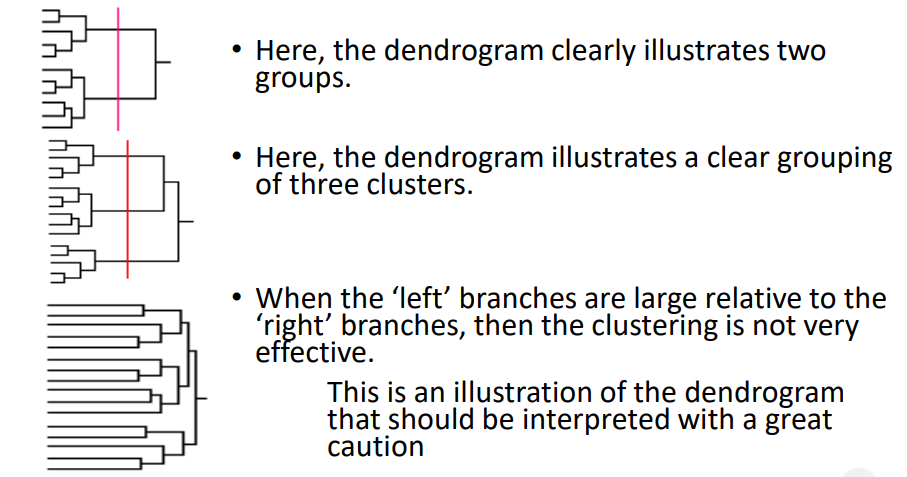
\includegraphics[width= \textwidth]{Images/Dendrograms.PNG}
    \caption{Interpreting a dendrogram}
    \label{fig:dendrogram}
\end{figure}
\smallskip
You should cut a tree when the gaps between the clusters is the largest.
\\\\
Interpretation of the clustering depends on the linkage method selected.
\subsubsection{Similarity}
There are many ways of measuring similarity between clusters the most common way is using Euclidean distance
\subsubsubsection{Euclidean Distance}
\begin{equation}
    d(x,y) = \sqrt{\sum_{i=1}^n (x_i - y_i)^2}
\end{equation}
\\\\
Euclidean distance is the standard measure for clustering.
\subsubsubsection{Squared Euclidean Distance}
\begin{equation}
    d(x,y) = \sum_{i=1}^n (x_i - y_i)^2
\end{equation}
\\\\
This helps to get dense clusters, if we were to plot the cluster in a multidimensional space, we would like them to be relatively dense aggregations of points, with small distance between points within clusters and big distances between clusters
\subsubsubsection{Cosine  similarity}
\begin{equation}
    sim(x,y) = \cos(\theta) = \frac{x\cdot y}{\lVert x \rVert\lVert y\rVert}
\end{equation}
\\\\
The more similar object the closer the points, Cosine is maximal for similar objects.
\subsubsubsection{Manhattan Block}
\begin{equation}
    d(x,y) = \lVert x-y \rVert = \sum_{i=1}^n \lVert x_i - y_i \rVert
\end{equation}
\\\\
The geometry has been used in regression analysis since the 18th century, and today is often referred to as LASSO.
\subsection{Cluster Analysis}
Possible problems with Euclidean and squared Euclidean distances is different scales for different variables, one way to get around this problem is to standardise the variables using the Z-score.
\\\\
Cluster analysis methods will always produce a grouping the groupings produceds by cluster analysis may ore may not be useful for classifying objects. There are many options for cluster analysis therefore we can mine the data trying different methods combining different distances and linkages to discover the structure in the data. 
\\\\
There are many example of successful application of cluster analysis to real problems a famous example, PRIZM system: In 1970s the company Claritas clustered neighbourhoods (U.S. zip codes) into forty different groups based on census information, such as population density, income, age, etc. This classification scheme, call PRIZM (Potential Rating Index for Zip Markets), has proven to be very useful in direct mail advertising, radio station formats, and decisions about where to locate stores.
\subsection{K-means: Non-hierarchical clustering}
This method differs from hierarchical clustering in many ways, the most obvious ways being 
\begin{itemize}
    \item There is no hierarchy, the data is partitioned instead
    \item You have to supply the number of clusters (k) into which you want to data to be grouped
\end{itemize}
This method is conceptually simple but computationally intensive
\begin{itemize}
    \item The cases are initially assigned randomly to the k clusters
    \item Cases are then moved around between clusters using an iterative method so that a classification is produced such that the clusters must be internally similar but externally dissimilar to the other clusters
    \item We stop when moving any more cases between clusters would make the clusters become more variable.
\end{itemize}
Cluster variability is measured with respect to their means for the classifying variables, hence the name k-means clustering. If more than one variable is used to define the clusters then the distances between clusters are measured in multi-dimensional space
\\\\
K-means is a relatively simple procedure, and consists of
choosing random k points that represent the distinct centres
of the k subsets, which are called centroids.
\begin{itemize}
    \item We then select, for each centroid, all the points closest to it
    \item This will create k different subsets.
    \item At this point, for each subset, we will re-calculate the centre
    \item We have again, k new centroids, and we repeat the steps above, selecting for each centroid, the new subsets of points closest to the centroids.
    \item  We continue this process until the centroids stop moving
\end{itemize}
For this technique to work, we need to be able to identify a metric that allows us to calculate the distance between points. This summarised as follows.
\begin{enumerate}
    \item Choose initial k-points, called centroids
    \item To each point in the data set, associate the closest centroid
    \item Calculate the new centre for the sets of points associated to a particular centroid
    \item Define the new centres to the new centroids
    \item Repeat steps 3 and 4 until the centroids stop moving
\end{enumerate}
\subsubsection{Silhouette}
Clustering results can be represented in a graphical form using silhouettes.
\\\\
The silhouette value for each point is a measure of how similar that point is to points in its own cluster, when compared to points in other clusters. The silhouette value for the  $i\;th$ point, $S_i$, is defined as
\begin{equation}
    S_i = \frac{b_i - a_i}{max(a_i,b_i)}
\end{equation}
Where $a_i$, is the average distance from the $i\;th$ point to the other points in the same cluster as $i$, and $b_i$ is the minimum average distance from the $i\;th$ point to points in a different cluster, minimised over clusters.
\\\\
The silhouette value ranges from -1 to +1, a high silhouette value for point $i$ indicates that this point is well-matched to its own cluster, and poorly-matched to neighboring clusters. If most points have a high silhouette value, then the clustering solution is appropriate. If many points have a low or negative silhouette value, then the clustering solution may have either too many or too few clusters. The silhouette clustering evaluation criterion can be used with any distance metric. The mean silhouette value can be used to estimate a quality of clustering.
\subsubsection{What to bear in mind}
It is important to notice that this method is extremely sensitive to the initial choice of random centroids, and that it may be a good idea to repeat the process for different initial choices. Also it is possible for some of the centroids not to be closest to any of the points ion the data-set reducing the number of subsets down from k.
\subsection{K Nearest Neighbour (KNN) Classifier}
This is a type of instance-based learning, or lazy learning, where the function is only approximated locally and all computation is deferred until classification. The KNN algorithm is among the simplest of all machine learning algorithms. The training examples are vectors in a multidimensional feature space each with a class label. The training phase of the algorithm consists only of storing the feature vectors and class labels of the training samples.  In the classification phase, k is a user-defined constant, and an unlabelled vector (a query or test point) is classified by assigning the label which is most frequent among the k training samples nearest to that query point.
\subsubsection{Algorithm summary}
\begin{itemize}
    \item A positive integer k is specified, along with a new sample
    \item We select the k entries in our database which are closest to the new sample
    \item We find the most common classification of these entries
    \item This is the classification we give the new sample
\end{itemize}
\subsubsection{Features of KNN}
KNN stores the entire training data-set which it uses as its representation, KNN does not learn any model and it makes predictions just-in-time by calculating the similarity between an input sample and each training instance.
\subsubsection{Pros and cons of KNN}
Pros
\begin{itemize}
    \item No assumptions about data — useful, for example, for nonlinear data
    \item Simple algorithm — to explain and understand/interpret
    \item High accuracy (relatively) — it is pretty high but not competitive in comparison to better supervised learning models
\end{itemize}
Cons
\begin{itemize}
    \item Computationally expensive —because the algorithm stores all of the training data
    \item High memory requirement
    \item Stores all (or almost all) of the training data
    \item Testing stage might be slow for large N
    \item Sensitive to irrelevant features and the scale of the data
\end{itemize}
\newpage
%\section{Supervised Learning}
A Neural networks are AI computational systems that are 'inspired' by biological neural systems. Their main feature is the abiblity to learn from the expericnece with using examples of classification.
\\\\
A single neuron is a linear classifier, classification can be thought as a way of separating the input data.


\subsection{Perceptron}
This is a machine learning algorithm that helps provide classified outcomes for computing. It dates back to the 1950s and represents a fundamental example of how machine learning algorithms work to develop data structure. This algorithms was invented by Frank Rosenblatt, it has an input and an output layer, a binary activation function. Update rule based on Hebbian learning: connections that are active at the same time are strengthen.
\\\\
The basic of the algorithm is four parts.
\begin{itemize}
    \item Setup: Weights are randomly assigned typically between -0.5 and 0.5
    \item Inputs: $x_1, x_2,..,x_n$; binary (0/1)
    \item Connection Strengths: $w_1,w_2,...,w_n$ and bias $\theta$
    \item Summation $ h = \sum_{i=1}^{n} w_i x_i$
    \item Output $y = f(h-\theta)$; binary: if $h > T$ then $y = 0$ else $y =1$
\end{itemize}
A Perceptron is a linear classification. Therefore the linear separator between two classes on a 2d plane is $x_2 = kx_1+b$ where $k = \frac{w_1}{w_2}$ as $x_2$ can be written as $x_2 = -\frac{w_1}{w_2}x_1 + \frac{\theta}{w_2}$
\subsubsection{Learning rule: training perceptron}
In a general case, to adjust weights $w$ and the bias $\theta$ of the perceptron, the learning (training) procedure is used. The training set includes many pairs, the input vector $x$ and the targeted output $t(x,t)$ We send one input vector $x$ to the perceptron adn the the actual output is $O$. The learning rule to adjust weights and bias is based on the difference (error) between the actual output $O$ and the targeted value $t:error = t-O$
\begin{itemize}
    \item Error: $e= t-O$
    \item $W_{new} = W_{old} +qx(t-O)$
    \item $\theta_{new} \theta_{old} + q(t-O)$
    \item Where $0<q<1$is the learning rate
\end{itemize}
This is also know as the Hebbian learning algorithms and mathematical equation is as follows.
\begin{equation}
    W_{ij}[n+1] = W_{ij}[n] + \eta x_i[n]x_j[n]
\end{equation}
Where $\eta$ is the learning rate coefficient and $x$ are the outputs of the $i$th and $j$th elements.
\subsubsection{Example}
Lets examine a simple example to help see how a perceptron can learn to represent the logical-OR function for two inputs, using a threshold of zero $t = 0$ and a learning rate $\eta$ of 0.2.
\begin{itemize}
    \item First we need set the associated weights which for this example will be $w_1 = -0.2$ and $w_2=0.4$
    \item Now, the first epoch is run through, the training data will consist of the four combinations of 1's and 0's possible with two inputs. Hence, our first piece of training data is $x_1 = 0$ and $x_2 = 0$ and our expected outcome is 0
    \item So we apply the formula $ h = \sum_{i=1}^{n} w_i x_i$
    \item resulting in $h = 0$
    \item since $h$ is as expected, and the error, $e$, is therefore 0, the weights do not change.
    \item Now $x_1 = 0$ and $x_2 =1$ and our expected outcome is 1
    \item Apply the formula and we get $h=0.4$
    \item So the output is 1, so the weights don't need to change
    \item Now $x_1 = 1$ and $x_2 =0$ and our expected outcome is 1
    \item Apply the formula and we get $h=-0.2$
    \item So the output is 0, so the weights need to change as the expected output was 1
    \item So we apply the perceptron training rule to assign new values to the weights, using the predefined $\eta$ and this case $e$ is 1.
    \item $w_1 = -0.2(0.2\cdot1\cdot1)$,  $w_1 = 0$
    \item $w_2 = 0.4(0.2\cdot0\cdot1)$,  $w_1 = 0.4$ as this did not contribute to this error it is not adjusted.
    \item Now $x_1 = 1$ and $x_2 =1$ and our expected outcome is 1
    \item Apply the formula and we get $h=0.4$
    \item So the output is 1, so the weights don't need to change
    \item This is the end of the first epoch, and at this point the method runs again and continues to repeat until all four piece of training data are classified correctly. 
\end{itemize}
\subsubsection{Limitations}
The exclusive OR function cannot be modeled using a perceptron. This is because the perceptrons can only learn to model functions that are linearly separable.
\subsection{Multilayer Perceptron}
An artificial neural network (ANN) consists of a set of interconnected nodes. ANN is able to receive inputs from the environment and to learn new behaviours (responses)
\subsubsection{ANN: forward pass} 
A ANN: forward pass is similar to a perceptron, the unit output is given by the weighted sum of the inputs, passed through an activation function. 
\begin{figure}[htbp]
    \centering
    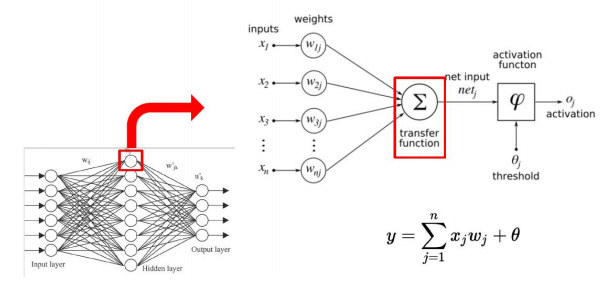
\includegraphics[width= \textwidth]{Images/ANNFowardPass.PNG}
    \caption{Hidden node}
    \label{fig`:dendrogram}
\end{figure}
\smallskip
\subsubsection{ANN: backward pass (error estimation)}
The performance of the network is evaluated using a loss function which must be differentiable. Generally an L2 norm is used the output is then compared with the expected value. The expected value is given by the label associated with the input and is stored in the data set. 
\begin{figure}[!htbp]
    \centering
    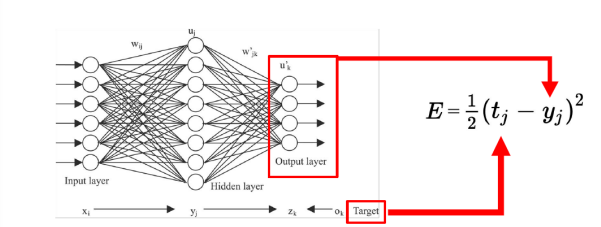
\includegraphics[width= \textwidth]{Images/OutputLayer.PNG}
    \caption{Output node}
    \label{fig`:dendrogram}
\end{figure}
\smallskip
\subsubsection{ANN: backward pass (update rule)}
The standard approach for training an ANN is back-propagation this is based on gradient descent, at each iteration the weights are adjusted in order to obtain an output that is more similar to the target. It is important to select the right hyper-parameters (e.g. learning rate).
\begin{figure}[!htbp]
    \centering
    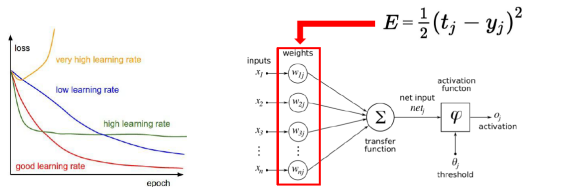
\includegraphics[width= \textwidth]{Images/UpdateRule.PNG}
    \caption{Update weights}
    \label{fig`:dendrogram}
\end{figure}
\smallskip
\subsubsection{Activation functions}
An activation function of a node defines the output of that node. It maps the resulting values into the desired range such as between 0 to 1 or -1 to 1 etc. (depending upon the choice of activation function). For example, the use of the logistic activation function would map all inputs in the real number domain into the range of 0 to 1, depending upon the choice of activation function.
\subsubsubsection{Sigmoid activation function}
This is a mathematical function that has the characteristic of an "S"-shaped curve. Often the sigmoid function refers to a special case of the logistic function. \\\\
The definition of a sigmoid functions is as follows. 
\begin{center}
    \textbf{A sigmoid function is bounded, differential, real function that is defined for all real input values and has a non-negative derivative at each point.}
\end{center}
In general, a sigmoid function is monotonic, and has a first derivative which is bell shaped. A sigmoid function is constrained by a pair of horizontal asymptotes as {\displaystyle x\rightarrow \pm \infty }
\subsubsection{ANN with hidden layers}
 The training data (input array and target output) should be
used to adjust parameters of ANN classifier,the learning procedure is based on minimization of the
total (for all training data) error function which depends on
training data and many parameters (weights and biases. Minimization is based on the idea of the gradient descend method. To minimize computational time, the idea of
backpropagation is used: moving backward (from output to input though several hidden layers) pick up already calculated components of the gradient and use them to
adjust ANN parameters.
\subsection{Support Vector Machine Binary Classifier}
Look at notes
\newpage
%\section{Problem Solving and Game Playing}
Problem solving is the study of AI algorithms that try and find the sequence of actions that lead to problem solution. There are several benchmark problems/games 
\begin{itemize}
    \item Travelling Salesperson Problem
    \item Missionaries and cannibals
    \item Crypto-arithmetic
    \item Games: Hanabi ,Starcraft2, Go, Chess and Tic-Tac-Toe
    \item Robot navigation
\end{itemize}
Some of these problems have been define as complex problems our have a layer of information hiding so the agent does not know all of the information.
\\\\
Key terms
\begin{itemize}
    \item Search space: The initail set of all possible conditions that satisfy the problem constraints
    \item Problem definition: A search tree which illustrates the initial, intermediate and goal states
    \item Search Strategy: A way to decide the next state to expand
\end{itemize}
\subsection{Graphs and Search Trees}
A graph is made of a set of nodes connected by links that may be directed or undirected, A successor is a neighbouring node that can be reached via a link, with a path being a sequence of nodes that connect two nodes together via links. A acyclic graph is a graph where no node has a path linking to itself, no cycles. Finally a tree is a type of graph where each node is connected by only one path. 
\subsection{Problem types}
There are two main problem types Single-state problem and Multiple-state problem. A Single-state problem is where all action consequences are known, whereas, a Multiple-state problem is when the environment is not fully accessible and only partial states are known to the agent.
\subsubsection{To solve problems}
To solve problems you need a set of initial conditions that will help define what a optimal and valid solution to the problem is.
\begin{itemize}
    \item Initial state and State space: Collection of all possible world states
    \item Operators: actions that lead to state change
    \item Goal test: A way to identify the goal state(s)
    \item Path cost: A function that is assigns a cost to a particular path
    \item Search trees: A Pathway between search states
    \item Search Strategy: To decide the next state to expand to.
\end{itemize}

\subsection{Search Algorithms}
There a two main types of search algorithms Blind search and Heuristic search. Blind search is and uninformed method and used where there is no information about the number of steps of the total path cost, whereas, Heuristic search is informed meaning that it is used when it is possible to know the relative cost of nodes.
\subsubsection{Blind Search Algorithms}
General Search algorithms are distinguished by the order in which nodes are expanded. A list that certainly is not exhaustive can be seen below.
\begin{itemize}
    \item Breadth-First Search: expands the shallowest node first
    \item Depth-First Search: expands the deepest node first
    \item Depth-Limited Search: puts a limit in the depth-first search
    \item Uniform Cost Search: expands the least operator-cost node first
\end{itemize}
\subsubsection{Heuristic Search}
For general AI a heuristic is any technique that improves the average performance on a problem solving task. A list of heuristic search algorithms that certainly is not exhaustive can be seen below.
\begin{itemize}
    \item Greedy Search: Best-first algorithm where the heuristic function defines the node cost.
    \item A* Search: Greedy search and the Uniform cost algorithm.
\end{itemize}
\subsection{Minimax Algorithm}
The minimax algorithm determines the optimal strategy for the \emph{Max} player by maximising its utility and assuming the  \emph{Min} player will play perfectly to minimise it.
\\\\
In tic-tac-toe this can be used using the two evaluating functions 
\begin{equation}
    3X_2 + X_1 - (3O_2+O_1)
\end{equation}
Where $X_n$ is the number of rows with n $X$ and no $O$.
\begin{equation}
    Open_{MAX} - Open_{MIN}
\end{equation}
Where $Open_{MAX}$ is the number of complete rows/columns/diagonals that are still open for MAX.
\newpage
%\input{notes/L6.tex}
\newpage
%\section{Evolutionary Computation}
Evolutionary Computation is the area of computer science interested in optimising solutions to problems that are often NP-hard, by using nature as the inspiration to for the techniques.
\subsection{Formal definition}
Given an optimisation problem $f(x)$, find a solution $x$ that optimises the function $f$. When the search space is simple this is not a very hard problem see figure \ref{fig:x^2}, whereas for search space is often not that nice!
\begin{figure}[!htbp]
    \centering
    \begin{tikzpicture}
      \draw[->] (-3,0) -- (3,0) node[right] {$x$};
      \draw[->] (0,-3) -- (0,5) node[above] {$y$};
      \draw[scale=0.5,domain=-3:3,smooth,variable=\x,blue] plot ({\x},{\x*\x});
    \end{tikzpicture}
    \caption{$f(x) = x^2$}
    \label{fig:x^2}
\end{figure}
\\\\
To optimise a problem we must consider a few very important things about the solution
\begin{itemize}
    \item representation 
    \item evaluation of quality
    \item illegal solutions are not generated
    \item they are generated from scratch
    \item modify
    \item a way to identify the best one
\end{itemize}
\newpage
%\section{Computer Vision}
Computer Vision is a field that deals with how computers can be made to gain a high level of understanding from images.
\subsection{Image Processing}
There are many different ways to process an image as shown below
\begin{itemize}
    \item Spatial filtering using Difference of Gaussians
    \begin{itemize}
        \item Low-pass 
        \item Band-pass
        \item High-pass
    \end{itemize}
    \item Illumination gradients
    \begin{itemize}
        \item Image differentiation -edges
        \item Sobel, Canny filters
    \end{itemize}
    \item Filtering in time
    \begin{itemize}
        \item Motion analysis
    \end{itemize}
\end{itemize}
All of these techniques use convolution 
\subsubsection{Convolution}
Convolution is the a mathematical operations on two functions $f$ and $g$ to produce a third function that expresses how the shape of one is modified by the other.
\\\\
\textbf{Definition}
\smallskip
\hrule
\bigskip
The convolution of $w$ and $v$ is written as $w*v$. It is defined as the integral of the product of the two functions are one is reversed and shifted. As such, it is a particular kind of integral transform.\footnote{For more  information about the definition with a visual explanation \href{https://en.wikipedia.org/wiki/Convolution}{(link)}  }
\[
(w*v)(x) \triangleq \int_{-\infty}^{\infty} w(\tau)v(x-\tau)d\tau
\]
\\
\subsubsubsection{Discrete Convolution}
\\\\
\textbf{Definition}
\smallskip
\hrule
\bigskip
For complex-valued functions, $f,g$ are defined on the set \mathbb{Z}, the discrete convolution of $f$ and $g$ is given by
\[
(f*g)[n] = \sum_{m = -\infty}^{\infty}f[m]g[n-m]
\]
or equivalently by
\[
(f*g)[n] = \sum_{m = -\infty}^{\infty}f[n-m]g[m]
\]
\\
So in images this method is used as images are represented in the \mathbb{Z} set.\footnote{To see a visual example of this working and a walk through \href{http://www.songho.ca/dsp/convolution/convolution2d_example.html}{(link)}} 
\subsubsection{Spatial filtering}
Spatial filtering is an technique for changing the intensities of a pixel according to the intensities of the neighboring pixels.
\subsubsubsection{Difference of two Gaussians (DoG)}
This is a symmetric band-pass filter, which removes high frequency components representing noise, and some low frequency components representing the homogeneous areas of the image. The frequency componets in the passing band are assumed to be associated to the edges in the images.
\\\\
The first step is to smooth the image by convolution with the Gaussian kernel of certain width ${\sigma_{1}}$
\[
G_{\sigma_{1}}(x,y) = \frac{1}{\sqrt{2\pi{\sigma_{1}}}}e^{-\frac{x^2+y^2}{2{\sigma_{1}}^2}}
\]
to get
\[
g_1(x,y) = G_{\sigma_{1}}(x,y) * f(x,y)
\]
with a different width ${\sigma_{2}}$, a second smoothed image can be obtained
\[
g_2(x,y) = G_{\sigma_{2}}(x,y) * f(x,y)
\]
We can now show that difference in these two Gaussian smoothed images can be used to detect edges in an image.

\[
g_1(x,y) - g_2(x,y) = G_{\sigma_1} * f(x,y) - G_{\sigma_2} * f(x,y) = (G_{\sigma_1} - G_{\sigma_2} * f(x,y) = DoG*f(x,y).
\]
The DoG as an operator is defined as \\\\
\textbf{Definition}
\smallskip
\hrule
\bigskip
\[
DoG \triangleq (G_{\sigma_1} - G_{\sigma_2}) = \frac{1}{\sqrt{2\pi}}\big(\frac{1}{\sigma_1}e^{-\frac{x^2+y^2}{2\sigma_1^2}}- \frac{1}{\sigma_2}e^{-\frac{x^2+y^2}{2\sigma_2^2}}\big) 
\]
\\
\subsubsubsection{Sobel gradient processing}
This operator uses two 3 by 3 kernels which are convoled with the original image to calculate approximations of the derivatives. If we define $A$ as the source image, and $G_x$ and $G_y$ are the two images which at each point contain the vertical and horizontal derivative approximations respectively. 

\[\centering
G_x = \begin{bmatrix} 
    -1&0&+1\\
    -2&0&+2\\
    -1&0&+1\\
    \end{bmatrix}
    * A
\]
\begin{center}
    and
\end{center}
\[ \centering
 G_y = \begin{bmatrix} 
    -1&-2&-1\\
    0&0&0\\
    +1&+2&+1\\
    \end{bmatrix}
    * A
\]
Since the Sobel kernels ca nbe decomposed as the products of an averaging and differentiation kernel, they compute the gradient with smoothing. At each point in the image the resulting gradient approximations can be combined to give the gradient magnitude.\footnote{For more information on this filtering technique visit \href{https://www.tutorialspoint.com/dip/sobel_operator.htm}{(link)}}
\[
G = \sqrt{G_x^2 + G_y^2}
\]
Using this we can calculate the gradients direction
\[
\theta = \arctan(\frac{G_y}{G_x})
\]

\newpage
\section{Formal Languages and Automata}
Pattern matching is central to many applications and supported by regular expressions in programming languages. The Chomsky hierarchy of Formal Languages provides a theory of programming languages of increasing expressively. Formal Automata or Machines are models of computation, that implement languages of the Chomsky hierarchy.
\subsection{Regular Expressions}
A regular expression describes a pattern, it has very basic operators however with these operations it can specify a usually infinite set of strings see table \ref{tab:regex}. \footnote{RegExp cheat sheet \href{https://www.cheatography.com/davechild/cheat-sheets/regular-expressions/}{(link)}}
\begin{table}[h]
\begin{tabular}{llll}
\hline
\multicolumn{1}{|l|}{\textbf{Operation}} & \multicolumn{1}{l|}{\textbf{Regular Expression}} & \multicolumn{1}{l|}{\textbf{Yes}} & \multicolumn{1}{l|}{\textbf{No}} \\ \hline
\multicolumn{1}{|l|}{Concatenation} & \multicolumn{1}{l|}{aabbaab} & \multicolumn{1}{l|}{aabaab} & \multicolumn{1}{l|}{Every Other String} \\ \hline
\multicolumn{1}{|l|}{Wildcard} & \multicolumn{1}{l|}{.u.u.u.} & \multicolumn{1}{l|}{\begin{tabular}[c]{@{}l@{}}cumulus\\ jugulum\end{tabular}} & \multicolumn{1}{l|}{\begin{tabular}[c]{@{}l@{}}succubus\\ tumultuous\end{tabular}} \\ \hline
\multicolumn{1}{|l|}{Union} & \multicolumn{1}{l|}{aa | baab} & \multicolumn{1}{l|}{\begin{tabular}[c]{@{}l@{}}aa\\ babb\end{tabular}} & \multicolumn{1}{l|}{Every Other String} \\ \hline
\multicolumn{1}{|l|}{Closure} & \multicolumn{1}{l|}{ab*a} & \multicolumn{1}{l|}{\begin{tabular}[c]{@{}l@{}}aa\\ abbba\end{tabular}} & \multicolumn{1}{l|}{\begin{tabular}[c]{@{}l@{}}ab\\ ababa\end{tabular}} \\ \hline
\multicolumn{1}{|l|}{\multirow{2}{*}{Parentheses}} & \multicolumn{1}{l|}{a(a|b)aab} & \multicolumn{1}{l|}{\begin{tabular}[c]{@{}l@{}}aaaab\\ abaab\end{tabular}} & \multicolumn{1}{l|}{Every Other String} \\ \cline{2-4} 
\multicolumn{1}{|l|}{} & \multicolumn{1}{l|}{(ab)*a} & \multicolumn{1}{l|}{\begin{tabular}[c]{@{}l@{}}a\\ ababababa\end{tabular}} & \multicolumn{1}{l|}{\begin{tabular}[c]{@{}l@{}}\varepsilon\\ abbbaa\end{tabular}} \\ \hline
\end{tabular}
\caption{Regex}
\label{tab:regex}
\end{table}
\subsubsection{Generalised Regular Expressions}
These have all of the rules previously mentioned however they also have more as seen in the table \ref{tab:Gregex}
\begin{table}[H]
\begin{tabular}{llll}
\hline
\multicolumn{1}{|l|}{\textbf{Operation}} & \multicolumn{1}{l|}{\textbf{Regular Expression}} & \multicolumn{1}{l|}{\textbf{Yes}} & \multicolumn{1}{l|}{\textbf{No}} \\ \hline
\multicolumn{1}{|l|}{One or more} & \multicolumn{1}{l|}{a(bc)+de} & \multicolumn{1}{l|}{\begin{tabular}[c]{@{}l@{}}abcde\\ abcbcde\end{tabular}} & \multicolumn{1}{l|}{\begin{tabular}[c]{@{}l@{}}ade\\ bcde\end{tabular}} \\ \hline
\multicolumn{1}{|l|}{Character classes} & \multicolumn{1}{l|}{{[}A-Za-z{]}{[}a-z{]}*} & \multicolumn{1}{l|}{\begin{tabular}[c]{@{}l@{}}capitalised\\ Word\end{tabular}} & \multicolumn{1}{l|}{\begin{tabular}[c]{@{}l@{}}camelCase\\ 4illegal\end{tabular}} \\ \hline
\multicolumn{1}{|l|}{Exactly k} & \multicolumn{1}{l|}{{[}0-9{]}\{5\}-{[}0-9{]}\{4\}} & \multicolumn{1}{l|}{\begin{tabular}[c]{@{}l@{}}08540-1321\\ 19072-5541\end{tabular}} & \multicolumn{1}{l|}{\begin{tabular}[c]{@{}l@{}}111111111111\\ 166-54-111\end{tabular}} \\ \hline
\multicolumn{1}{|l|}{Negations} & \multicolumn{1}{l|}{{[}\textasciicircum{}aeiob{]}\{6\}} & \multicolumn{1}{l|}{rhythm} & \multicolumn{1}{l|}{decade} \\ \hline
\multirow{2}{*}{} &  &  &  \\
\end{tabular}
\caption{Generalised Regex}
\label{tab:Gregex}
\end{table}
\subsection{Deterministic Finite State Automata (DFA)}
A DFA $M$ is  a 5-tuple $M= \{Q,\Sigma,q_0,F,\delta\}$ where 
\begin{itemize}
    \item $Q$ is a finite set of states
    \item $\Sigma$ is finite set of input symbols ("alphabet")
    \item $q_0$ is a start state from $Q$
    \item F is a set of accepting states from $Q$
    \item $\delta$ is a transition function, i.e. a total mapping from $Q\times\Sigma$ to $Q$
\end{itemize}
\subsubsection{Transition Function}
The transition function $\delta$ takes a state $q$ and an input symbol $a$ and maps them to a state $q'$. The function is 'total' for each pair $(q,a)$ exactly one target state $q$ must exist so $\delta(q,a)=q'$ this function is often written as $q \xrightarrow{a}q'$. $\delta$ can be represented by a matrix $T$ in code.
\subsubsection{Example of what the symbols mean}
Using the figure \ref{fig:DFAB*} and calling it $M$ so $M= \{Q,\Sigma,q_0,F,\delta\}$ the symobls represent
\begin{itemize}
    \item $Q$ is $q_0,q_1$
    \item $\Sigma$ is a,b
    \item $q_0$ is $q_0$
    \item F is $q_0$
    \item $\delta(q_0,a) = q_1$, $\delta(q_0,b) = q_0$, $\delta(q_1,a) = q_1$, $\delta(q_1,b) = q_1$
\end{itemize}
\begin{figure}[H]
    \centering
  \begin{tikzpicture}[shorten >=1pt,node distance=2cm,on grid,auto] 
   \node[state,initial,accepting] (q_0)   {$q_0$}; 
   \node[state] (q_1) [right=of q_0] {$q_1$}; 
    \path[->] 
    (q_0) edge  node {a} (q_1)
          edge [loop above] node {b} ()
    (q_1) edge  [loop above] node {a,b} ();
  \end{tikzpicture} 
    \caption{DFA of regex b*}
    \label{fig:DFAB*}
\end{figure}
\subsubsection{How a DFA Works}
A run of a DFA $M$ on $s$ = $a_0,a_1,..,a_{n-1}$ is a sequence of states $q_0,q_1,q_2,..,q_n$ such that $q_i \xrightarrow{a}q_{i+1}\,\, \forall \,\, 0\leq i \le n$. The determinism part means for a given input word a DFA has a unique run, because the transition function is a total function. A DFA accepts a word if $q_n$ is in the set of final state $F$; otherwise it rejects the word.
\subsubsection{Informal definition}
In figure \ref{fig:DFSA} the DFA has three states $q_0$,$q_1$ and $q_2$ with $q_1$ being the goal state and $q_0$ being the start state.
\begin{figure}[H]
    \centering
  \begin{tikzpicture}[shorten >=1pt,node distance=2cm,on grid,auto] 
   \node[state,initial] (q_0)   {$q_0$}; 
   \node[state,accepting] (q_1) [above right=of q_0] {$q_1$}; 
   \node[state] (q_2) [below right=of q_0] {$q_2$}; 
    \path[->] 
    (q_0) edge  node {a} (q_1)
          edge  node [swap] {b} (q_2)
    (q_1) edge [loop above] node {a,b} ()
    (q_2) edge [loop below] node {a,b} ();
\end{tikzpicture} 
    \caption{DFA}
    \label{fig:DFSA}
\end{figure}
The DFA in figure \ref{fig:DFSA} reads inputs symbols as a's or b's and transits between states as indicated by the labelled arrows. 
\\\\
In a DFA there can only be one starting state however there can be multiple goal states which is represented as by the double circle. Once an all inputs have been read if the end state is a goal state then the string is correct/accepted otherwise it is wrong/rejected. 
\subsubsection{Pseudo code}
\begin{algorithm}[H]
\SetAlgoLined
\KwResult{True or False }
 T = [1,0;1,1]\;
 
 q = $q_0$\;
 
 a = $a_0,a_1,..,a_{n-1}$\;
 
 \\
 \While{$i$ $\le$ $N-1$}{
    q = T[q,a[i]]\;
 }
\eIf{q is in $F$}{
return True\;
}{
return False\;
}
 \caption{DFA Algorithms}
\end{algorithm}
\subsection{Non-Deterministic Finite State Automata (NFA)}
In a DFA, each pair of state and input symbol uniquely defines a next state, however, in Non-determinism allows for missing and non-unique transitions (and possibly for more than 1 start state). If multiple targets exist (non-determinism!) the machine is “cloned” and all alternatives run further. There may be “epsilon-transitions” (without an input). If a target state cannot be determined the machine dies
A word is accepted if at least one derivation exists, i.e. if at least
one machine survives in an accepting state.
\subsubsection{NFA example}
The NFA figure \ref{fig:NFA*} can have multiple runs with the same word for example $abbb$ can end up in either $s_1$ or $s_2$. An NFA can have 0,1 or more than one runs on a given word.
\begin{figure}[H]
    \centering
  \begin{tikzpicture}[shorten >=1pt,node distance=2cm,on grid,auto] 
   \node[state,initial] (s_1)   {$s_1$}; 
   \node[state,accepting] (s_2) [right=of s_1] {$s_2$}; 
    \path[->] 
    (s_1) edge  node {b} (s_2)
          edge [loop above] node {a,b} ()
    (s_2) edge  [loop above] node {b} ();
  \end{tikzpicture} 
    \caption{NFA of words ending in b}
    \label{fig:NFA*}
\end{figure}
\subsection{Formal Languages}
Finite state machines accept or reject words, the set of all words an FSA called A accepts is called the Language it accepts 
\begin{equation}
    L(A) = \{u \in \Sigma^* \,\,|\,\, A \text{ has an accepting run on }u\}
\end{equation}
Regular Expressions characterise words as well, thereby they also define Languages.
\subsubsection{Equivalence (without proofs)}
For each DFA exists a regular expression that defines the same Language as the DFA.For each regular expression exists a DFA that accepts the same language as the RegExp For each NFA exists a DFA that accepts the same language (i.e. NFAs are not stronger than DFAs) DFAs, NFAs, and regular expressions all compute the same class of languages. These are the regular languages
\subsection{Grammars and Languages}
A Formal Grammer is a 4 tuple $G(V,\Sigma,P,S$

\end{document}
